\documentclass{aa}

% \usepackage[utf8x]{inputenc}
% \usepackage[T1]{fontenc}
% \usepackage{txfonts, natbib}
\usepackage{amsmath, amsfonts, amssymb}
\usepackage{graphicx}

\begin{document}

\title{Reflections on the Decline of Science in England, and on Some of Its Causes \thanks{This was shamelessly copied from Project Gutemberg}}

\author{
    E. T. Barrionovo\inst{1}
    \and C. Babbage \inst{2}
}

\offprints{E. T. Barrionovo}

\institute{OV \and Trinity College}

\titlerunning{Decline of Science in England}
\authorrunning{E. T. Barrionovo et al.}

\date{Received date; accepted date}

\abstract
% context
{Of the causes which have induced me to print this volume I have little
to say; my own opinion is, that it will ultimately do some service
to science, and without that belief I would not have undertaken so
thankless a task.}
% aims
{If any one shall endeavour to account for the opinions stated in these
pages by ascribing them to any imagined circumstance peculiar to myself,
I think he will be mistaken. That science has long been neglected and
declining in England, is not an opinion originating with me, but is
shared by many, and has been expressed by higher authority than mine.}
% methods
{The last authority which I shall adduce is more valuable, from the
varied acquirements of its author, and from the greater detail into
which he enters.}
% results
{Whatever may be the fate of that highly interesting document, we may
infer his opinions upon this subject from a sentiment expressed in his
last work}
% conclusion
{In concluding this most circumscribed outline of the History of
Chemistry, we may perhaps be allowed to express a faint shade of regret,
which, nevertheless, has frequently passed over our minds within the
space of the last five or six years.}

\keywords{Science -- Decline}

\maketitle


\section{Preface}

\label{preface}

Alguns artigos [\cite{cox}] sao mamilicos.

Of the causes which have induced me to print this volume I have little
to say; my own opinion is, that it will ultimately do some service
to science, and without that belief I would not have undertaken so
thankless a task. That it is too true not to make enemies, is an opinion
in which I concur with several of my friends, although I should hope
that what I have written will not give just reason for the permanence of
such feelings. On one point I shall speak decidedly, it is not connected
in any degree with the calculating machine on which I have been engaged;
the causes which have led to it have been long operating, and would have
produced this result whether I had ever speculated on that subject, and
whatever might have been the fate of my speculations.

If any one shall endeavour to account for the opinions stated in these
pages by ascribing them to any imagined circumstance peculiar to myself,
I think he will be mistaken. That science has long been neglected and
declining in England, is not an opinion originating with me, but is
shared by many, and has been expressed by higher authority than mine. I
shall offer a few notices on this subject, which, from their scattered
position, are unlikely to have met the reader's attention, and which,
when combined with the facts I have detailed in subsequent pages, will
be admitted to deserve considerable attention. The following extract
from the article Chemistry, in the Encyclopaedia Metropolitana, is from
the pen of a gentleman equally qualified by his extensive reading, and
from his acquaintance with foreign nations, to form an opinion entitled
to respect. Differing from him widely as to the cause, I may be
permitted to cite him as high authority for the fact.


\section{On the reciprocal influence of science and education}

That the state of knowledge in any country will exert a directive
influence on the general system of instruction adopted in it, is a
principle too obvious to require investigation. And it is equally
certain that the tastes and pursuits of our manhood will bear on them
the traces of the earlier impressions of our education. It is therefore
not unreasonable to suppose that some portion of the neglect of science
in England, may be attributed to the system of education we pursue. A
young man passes from our public schools to the universities, ignorant
almost of the elements of every branch of useful knowledge; and at these
latter establishments, formed originally for instructing those who
are intended for the clerical profession, classical and mathematical
pursuits are nearly the sole objects proposed to the student's ambition.

Much has been done at one of our universities during the last fifteen
years, to improve the system of study; and I am confident that there
is no one connected with that body, who will not do me the justice to
believe that, whatever suggestions I may venture to offer, are prompted
by the warmest feelings for the honour and the increasing prosperity of
its institutions. The ties which connect me with Cambridge are indeed of
no ordinary kind.

Taking it then for granted that our system of academical education ought
to be adapted to nearly the whole of the aristocracy of the country, I
am inclined to believe that whilst the modifications I should propose
would not be great innovations on the spirit of our institutions, they
would contribute materially to that important object.

\begin{equation}
    \oint_{\textsf{\textit{a}}}^{x_\phi} \sinh \frac{1 - \sqrt{\mu}}{\nabla^2\varpi} \, \textsf{\textit{d}}\varpi
    \label{IntegralBolada}
\end{equation}

It will be readily admitted, that a degree conferred by an university,
ought to be a pledge to the public that he who holds it possesses a
certain quantity of knowledge. The progress of society has rendered
knowledge far more various in its kinds than it used to be; and to meet
this variety in the tastes and inclinations of those who come to us for
instruction, we have, besides the regular lectures to which all must
attend, other sources of information from whence the students may
acquire sound and varied knowledge in the numerous lectures on
chemistry, geology, botany, history, \&c. It is at present a matter of
option with the student, which, and how many of these courses he shall
attend, and such it should still remain. All that it would be necessary
to add would be, that previously to taking his degree, each person
should be examined by those Professors, whose lectures he had attended.
The pupils should then be arranged in two classes, according to their
merits, and the names included in these classes should be printed. I
would then propose that no young man, except his name was found amongst
the "List of Honours," should be allowed to take his degree, unless he
had been placed in the first class of some one at least of the courses
given by the professors. But it should still be imperative upon the
student to possess such mathematical knowledge as we usually require. If
he had attained the first rank in several of these examinations, it
is obvious that we should run no hazard in a little relaxing: the
strictness of his mathematical trial.

\begin{figure*}
    \resizebox{\hsize}{!}{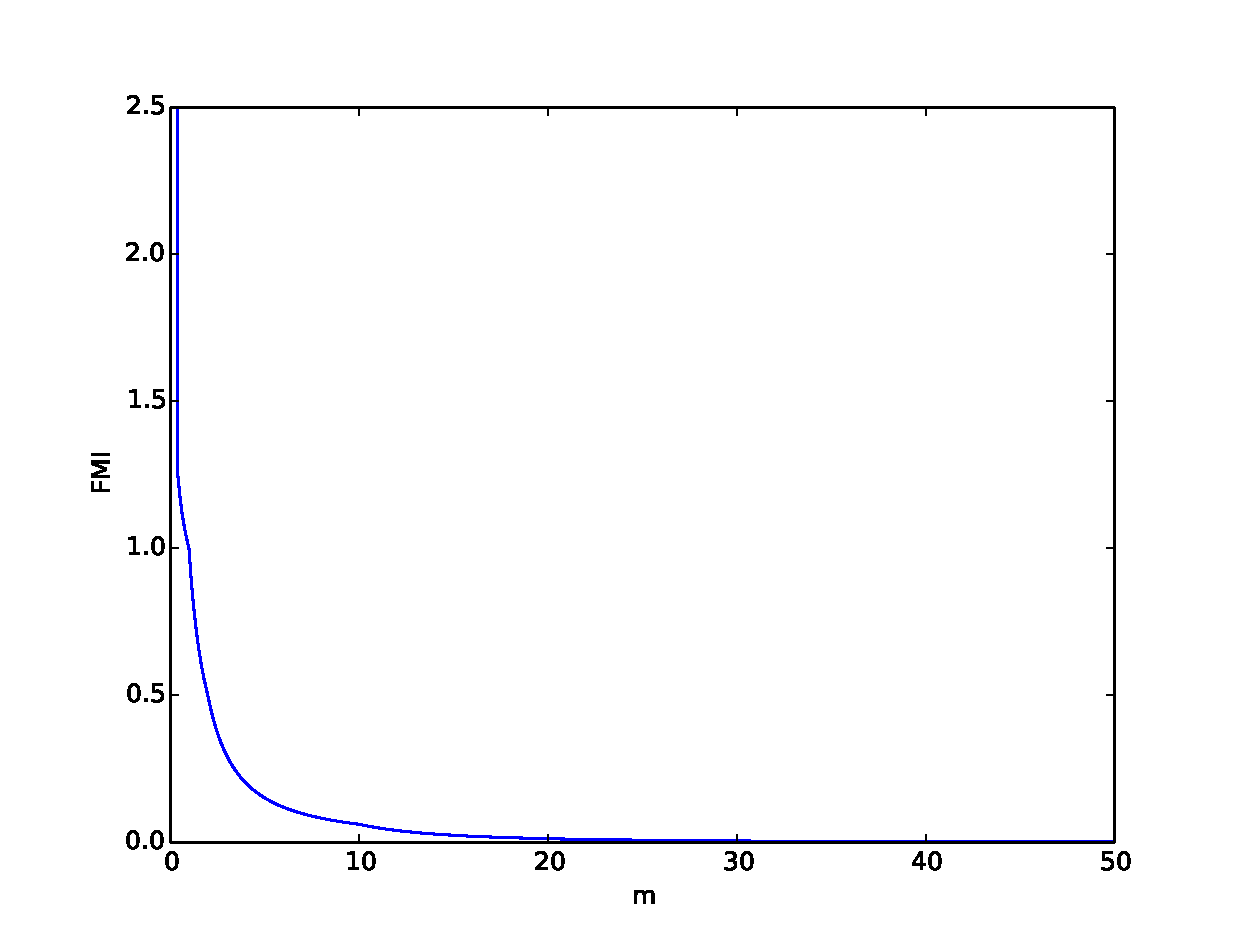
\includegraphics{figs/f4.eps}}'
    \caption[]{Quase exponencial}
    \label{QuaseExp}
\end{figure*}

One of the great advantages of such a system would be, that no young
person would have an excuse for not studying, by stating, as is most
frequently done, that the only pursuits followed at Cambridge, classics
and mathematics, are not adapted either to his taste, or to the wants of
his after life. His friends and relatives would then reasonably expect
every student to have acquired distinction in SOME pursuit. If it should
be feared that this plan would lead to too great a diversity of pursuits
in the same individual, a limitation might be placed upon the number of
examinations into which the same person might be permitted to enter. It
might also be desirable not to restrict the whole of these examinations
to the third year, but to allow the student to enter on some portion of
them in the first or second year, if he should prefer it.

Vide equacao \ref{IntegralBolada} e Fig. \ref{ztrend}.

By such an arrangement, which would scarcely interfere seriously with
our other examinations, we should, I think, be enabled effectually to
keep pace with the wants of society, and retaining fully our power
and our right to direct the studies of those who are intended for the
church, as well as of those who aspire to the various offices connected
with our academical institutions; we should, at the same time, open
a field of honourable ambition to multitudes, who, from the exclusive
nature of our present studies, leave us with but a very limited addition
to their stock of knowledge.

Much more might be said on a subject so important to the interests of
the country, as well as of our university, but my wish is merely to open
it for our own consideration and discussion. We have already done so
much for the improvement of our system of instruction, that public
opinion will not reproach us for any unwillingness to alter. It is our
first duty to be well satisfied that we can improve: such alterations
ought only to be the result of a most mature consideration, and of a
free interchange of sentiments on the subject, in order that we may
condense upon the question the accumulated judgment of many minds.

It is in some measure to be attributed to the defects of our system of
education, that scientific knowledge scarcely exists amongst the
higher classes of society. The discussions in the Houses of Lords or of
Commons, which arise on the occurrence of any subjects connected with
science, sufficiently prove this fact, which, if I had consulted the
extremely limited nature of my personal experience, I should, perhaps,
have doubted.


\section{Of the inducements to individuals to cultivate science}

Interest or inclination form the primary and ruling motives in this
matter: and both these exert greater or less proportionate influence in
each of the respective cases to be examined.

\subsection{Professional impulses}

A large portion of those who are impelled by ambition or necessity to
advance themselves in the world, make choice of some profession in which
they imagine their talents likely to be rewarded with success; and there
are peculiar advantages resulting to each from this classification of
society into professions. The ESPRIT DE CORPS frequently overpowers the
jealousy which exists between individuals, and pushes on to advantageous
situations some of the more fortunate of the profession; whilst, on the
other hand, any injury or insult offered to the weakest, is redressed or
resented by the whole body. There are other advantages which are perhaps
of more importance to the public. The numbers which compose the learned
professions in England are so considerable, that a kind of public
opinion is generated amongst them, which powerfully tends to repress
conduct that is injurious either to the profession or to the public.
Again, the mutual jealousy and rivalry excited amongst the whole body
is so considerable, that although the rank and estimation which an
individual holds in the profession may be most unfairly appreciated,
by taking the opinion of his rival; yet few estimations will be found
generally more correct than the opinion of a whole profession on the
merits of any one of its body. This test is of great value to the
public, and becomes the more so, in proportion to the difficulty of the
study to which the profession is devoted. It is by availing themselves
of it that men of sense and judgment, who have occasion for the services
of professional persons, are, in a great measure, guided in their
choice.

\begin{tabular}[t]{|l|ccccc|c|}
    \multicolumn{7}{c}{Notas das listas de exercícios} \\
    \hline
    Nome & L1 & L2 & L3 & L4 & L5 & Média \\
    \hline
    Zé Qualquer & 5 & 5 & 3 & 2 & 1 & 3.2 \\
    Zé Ninguém  & 5 & 5 & 5 & 4 & 5 & 4.8 \\
    Fulaninha   & 5 & 5 & 5 & 5 & 5 & 5.0\\
    \hline
\end{tabular}

The pursuit of science does not, in England, constitute a distinct
profession, as it does in many other countries. It is therefore, on
that ground alone, deprived of many of the advantages which attach
to professions. One of its greatest misfortunes arises from this
circumstance; for the subjects on which it is conversant are so
difficult, and require such unremitted devotion of time, that few who
have not spent years in their study can judge of the relative knowledge
of those who pursue them. It follows, therefore, that the public, and
even that men of sound sense and discernment, can scarcely find means
to distinguish between the possessors of knowledge, in the present
day, merely elementary, and those whose acquirements are of the highest
order. This remark applies with peculiar force to all the more difficult
applications of mathematics; and the fact is calculated to check the
energies of those who only look to reputation in England.

Veja secao \ref{preface}.

As there exists with us no peculiar class professedly devoted to
science, it frequently happens that when a situation, requiring for the
proper fulfilment of its duties considerable scientific attainments, is
vacant, it becomes necessary to select from among amateurs, or rather
from among persons whose chief attention has been bestowed on other
subjects, and to whom science has been only an occasional pursuit.
A certain quantity of scientific knowledge is of course possessed by
individuals in many professions; and when added to the professional
acquirements of the army, the navy, or to the knowledge of the merchant,
is highly meritorious: but it is obvious that this may become, when
separated from the profession, quite insignificant as the basis of a
scientific reputation.

\begin{equation}
    \frac{1}{2} < \left\lfloor \textnormal{mod} \left( \left\lfloor \frac{y}{17} \right\rfloor 2^{-17\left\lfloor x \right\rfloor - \textnormal{mod}\left( \left\lfloor y \right \rfloor ,  17 \right)}, 2 \right) \right\rfloor
    \label{Quine}
\end{equation}

To those who have chosen the profession of medicine, a knowledge of
chemistry, and of some branches of natural history, and, indeed, of
several other departments of science, affords useful assistance. Some of
the most valuable names which adorn the history of English science have
been connected with this profession.

The causes which induce the selection of the clerical profession are
not often connected with science; and it is, perhaps, a question of
considerable doubt whether it is desirable to hold out to its members
hopes of advancement from such acquirements. As a source of recreation,
nothing can be more fit to occupy the attention of a divine; and our
church may boast, in the present as in past times, that the domain of
science has been extended by some of its brightest ornaments.


\begin{equation}
    \cfrac{2}{1 + \cfrac{2}{1 + \cfrac{2}{1 + \cfrac{2}{1}}}}
    \label{Fracao}
\end{equation}


In England, the profession of the law is that which seems to hold out
the strongest attraction to talent, from the circumstance, that in it
ability, coupled with exertion, even though unaided by patronage, cannot
fail of obtaining reward. It is frequently chosen as an introduction
to public life. It also presents great advantages, from its being a
qualification for many situations more or less remotely connected
with it, as well as from the circumstance that several of the highest
officers of the state must necessarily have sprung from its ranks.

A powerful attraction exists, therefore, to the promotion of a study and
of duties of all others engrossing the time most completely, and which
is less benefited than most others by any acquaintance with science.
This is one amongst the causes why it so very rarely happens that men in
public situations are at all conversant even with the commonest branches
of scientific knowledge, and why scarcely an instance can be cited of
such persons acquiring a reputation by any discoveries of their own.

But, however consistent other sciences may be with professional
avocations, there is one which, from its extreme difficulty, and the
overwhelming attention which it demands, can only be pursued with
success by those whose leisure is undisturbed by other claims. To be
well acquainted with the present state of mathematics, is no easy task;
but to add to the powers which that science possesses, is likely to be
the lot of but few English philosophers.

\subsection{Of national encouragement}


The little encouragement which at all previous periods has been afforded
by the English Government to the authors of useful discoveries, or of
new and valuable inventions, is justified on the following grounds:


\begin{itemize}
    \item The public, who consume the new commodity or profit by the new
invention, are much better judges of its merit than the government can
be.

    \item The reward which arises from the sale of the commodity is usually
much larger than that which government would be justified in bestowing;
and it is exactly proportioned to the consumption, that is, to the want
which the public feel for the new article.
\end{itemize}


\begin{figure}
    \resizebox{\hsize}{!}{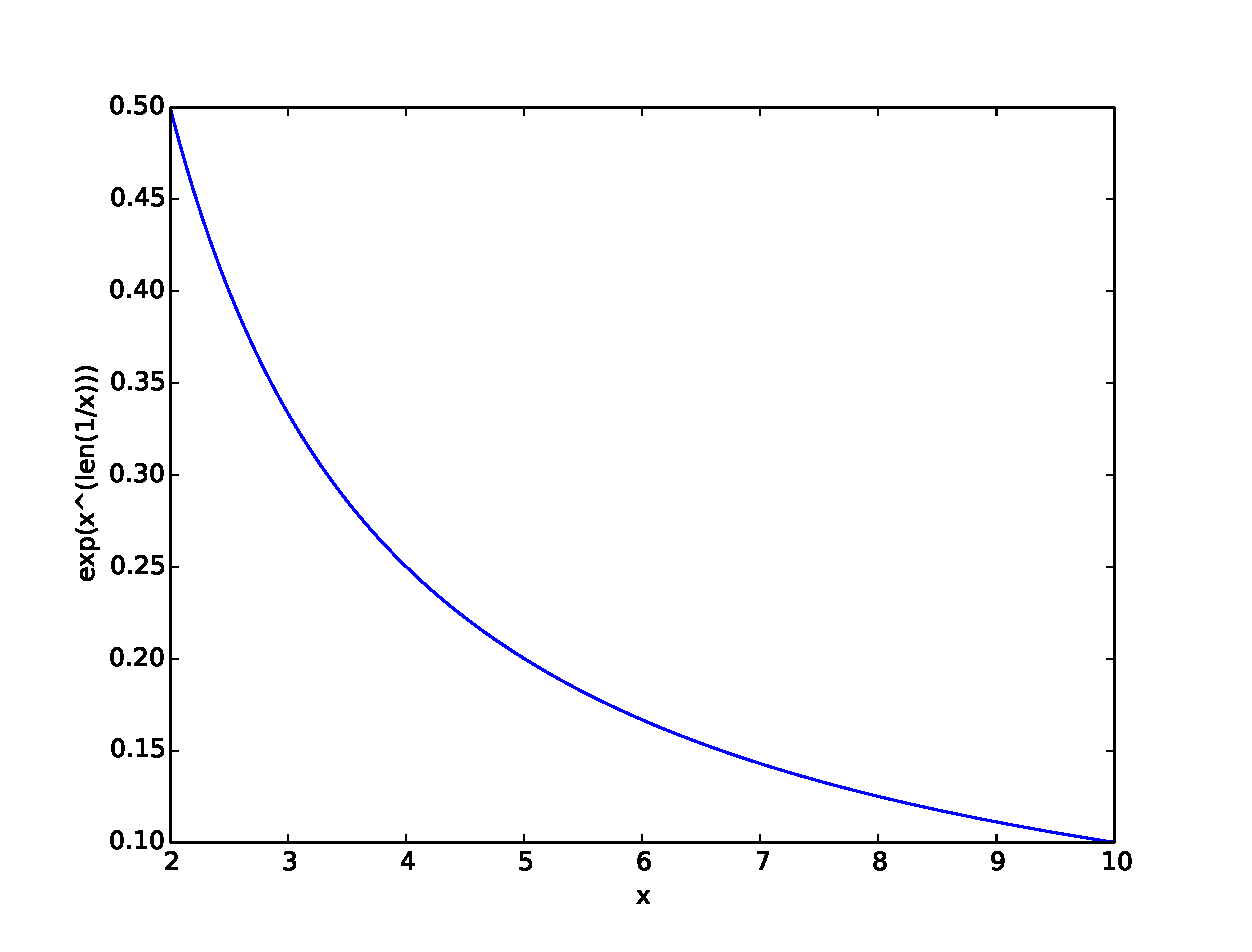
\includegraphics{figs/f2.eps}}'
    \caption[]{Exponencial}
    \label{ztrend}
\end{figure}


It must be admitted that, as general principles, these are correct:
there are, however, exceptions which flow necessarily from the very
reasoning from which they were deduced. Without entering minutely into
these exceptions, it will be sufficient to show that all abstract truth
is entirely excluded from reward under this system. It is only the
application of principles to common life which can be thus rewarded.
A few instances may perhaps render this position more evident. The
principle of the hydrostatic paradox was known as a speculative truth
in the time of Stevinus; [About the year 1600] and its application to
raising heavy weights has long been stated in elementary treatises on
natural philosophy, as well as constantly exhibited in lectures. Yet, it
may fairly be regarded as a mere abstract principle, until the late Mr.
Bramah, by substituting a pump instead of the smaller column, converted
it into a most valuable and powerful engine.--The principle of the
convertibility of the centres of oscillation and suspension in the
pendulum, discovered by Huygens more than a century and a half ago,
remained, until within these few years, a sterile, though most elegant
proposition; when, after being hinted at by Prony, and distinctly
pointed out by Bonenberger, it was employed by Captain Kater as the
foundation of a most convenient practical method of determining the
length of the pendulum.--The interval which separated the discovery, by
Dr. Black, of latent heat, from the beautiful and successful application
of it to the steam engine, was comparatively short; but it required the
efforts of two minds; and both were of the highest order.--The influence
of electricity in producing decompositions, although of inestimable
value as an instrument of discovery in chemical inquiries, can hardly be
said to have been applied to the practical purposes of life, until the
same powerful genius which detected the principle, applied it, by
a singular felicity of reasoning, to arrest the corrosion of the
copper-sheathing of vessels. That admirably connected chain of
reasoning, the truth of which is confirmed by its very failure as a
remedy, will probably at some future day supply, by its successful
application, a new proof of the position we are endeavouring to
establish.

\begin{thebibliography}{}

  \bibitem[1966]{baker} Baker, N. 1966,
      in Stellar Evolution,
      ed.\ R. F. Stein,\& A. G. W. Cameron
      (Plenum, New York) 333

   \bibitem[1988]{balluch} Balluch, M. 1988,
      A\&A, 200, 58

   \bibitem[1980]{cox} Cox, J. P. 1980,
      Theory of Stellar Pulsation
      (Princeton University Press, Princeton) 165

   \bibitem[1969]{cox69} Cox, A. N.,\& Stewart, J. N. 1969,
      Academia Nauk, Scientific Information 15, 1

   \bibitem[1980]{mizuno} Mizuno H. 1980,
      Prog. Theor. Phys., 64, 544

   \bibitem[1987]{tscharnuter} Tscharnuter W. M. 1987,
      A\&A, 188, 55

   \bibitem[1992]{terlevich} Terlevich, R. 1992, in ASP Conf. Ser. 31,
      Relationships between Active Galactic Nuclei and Starburst Galaxies,
      ed. A. V. Filippenko, 13

   \bibitem[1980a]{yorke80a} Yorke, H. W. 1980a,
      A\&A, 86, 286

   \bibitem[1997]{zheng} Zheng, W., Davidsen, A. F., Tytler, D. \& Kriss, G. A.
      1997, preprint
\end{thebibliography}

\end{document}
